\section{Nonlinear Regression}
\subsection{Prior Works}
\begin{frame}{Approximation Method}
  \begin{itemize}
    \item 2nd Order Volterra Kernel \cite{Friston2000}
    \note{Quadratic Approximation}
    \begin{itemize}
        \item Quadratic Convolution used to approximate Jacobian Matrix.
        \note{Because of the nonlinearities in the BOLD model, step size for
                integrating would otherwise be extremely small}
        \item Volterra approximation quality is not known.
    \end{itemize}
    \note{Volterra Approximation depends on sparsity etc}
    {\footnotesize
    $$y(t) = k_0 + \int_{-\infty}^{\infty} k_1(s_1) x(t-s_1) ds_1
        + \int_{-\infty}^{\infty} k_2(s_1,s_2) x(t-s_1)x(t-s_2) ds_1 ds_2$$
        \note{Its possible this isn't even knowable}
    }
    \item Canonical Hemodynamic Response Function
    \note{Linear Approximation}
    \begin{itemize}
        \item No Parameters Estimated
        \item Maximum Likelihood Possible
        \item Inflexible - even to changes in onset time
    \end{itemize}
    \begin{center}
    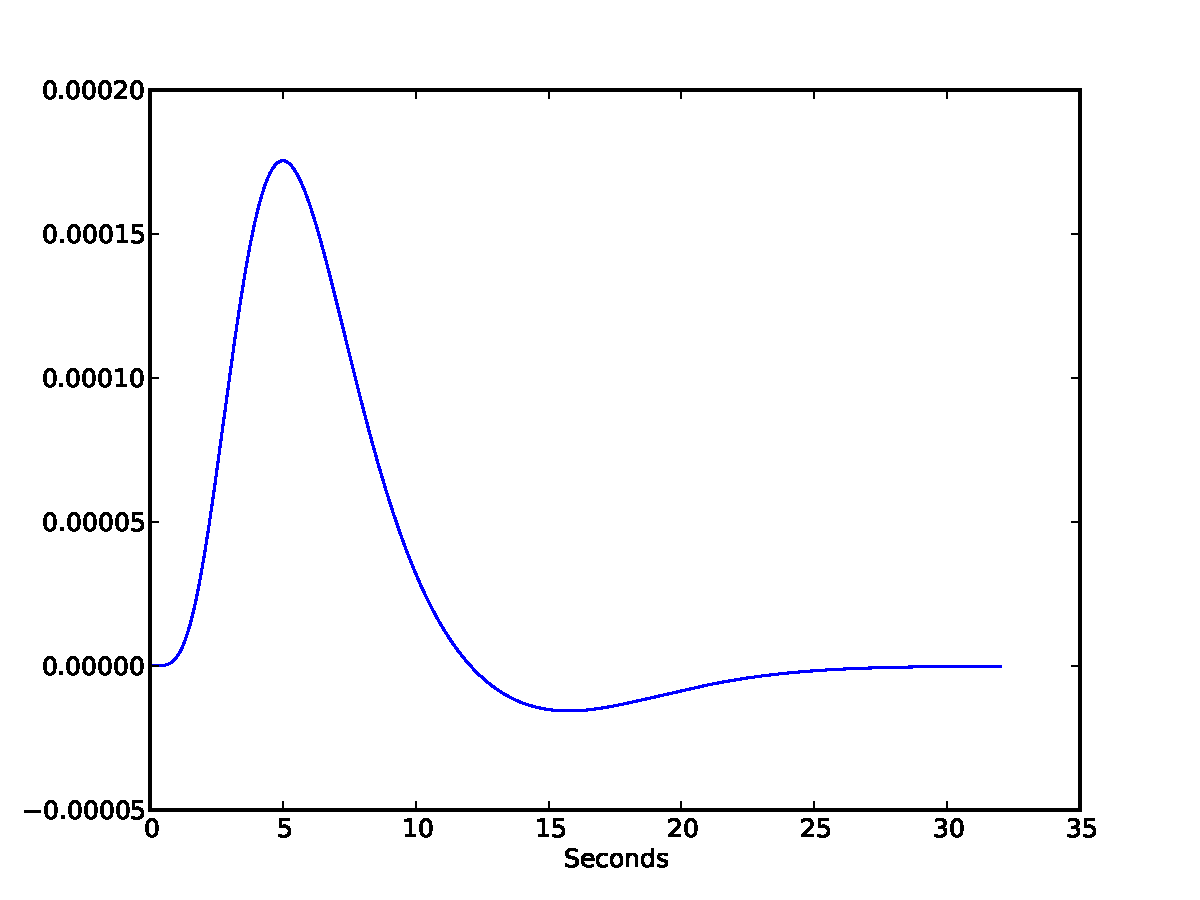
\includegraphics[clip=true,trim=4.88cm 0cm 5cm 1.5cm,height=2.7cm,width=8cm]{HRF}
    \end{center}
    
  \end{itemize}
\end{frame}

\begin{frame}{Nonlinear Methods}
\begin{itemize}
    \begin{columns}
    \begin{column}{.42\textwidth}
    \item Local Linearization filter, \cite{Riera2003}
    $$f(t)- f(t-1) \sim N(0, \sigma^2)$$
     \note{Jacobian of the $\dot{x}$ is available, making gradient descent possible}
    \item Genetic Algorithms and Simulated Annealing, \cite{Vakorin2007}
     \note{Genetic Algorithms were used to optimize spike points, simulated annealing for the parameters}
    \item Particle Filters to estimate States, \cite{Murray2009}
    \begin{itemize}
        \item ML estimate of $\Theta$, \cite{Johnston2007}
         \note{Particle Filter used to estimate states, ML of parameters based on the posterior of states and so on}
    \end{itemize}
    \item Unscented Kalman Filter \cite{Hu2009}
     \note{Technically Kalman Filters and Particle Filters are Bayesian Filters}
     \note{Essentially filtering out inconsistent parameters.}
    \end{column}

    \begin{column}{.58\textwidth}
    \begin{figure}
    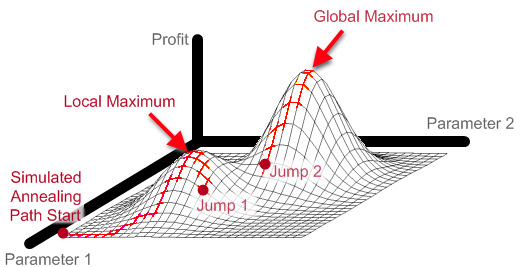
\includegraphics[clip=true,trim=0cm 0cm 0cm 1cm,width=.6\textwidth]{simulated_annealing}
    \caption{Simulated Annealing can escape local minima with chaotic jumps. \cite{Dama}}
    \end{figure}
    \begin{figure}
    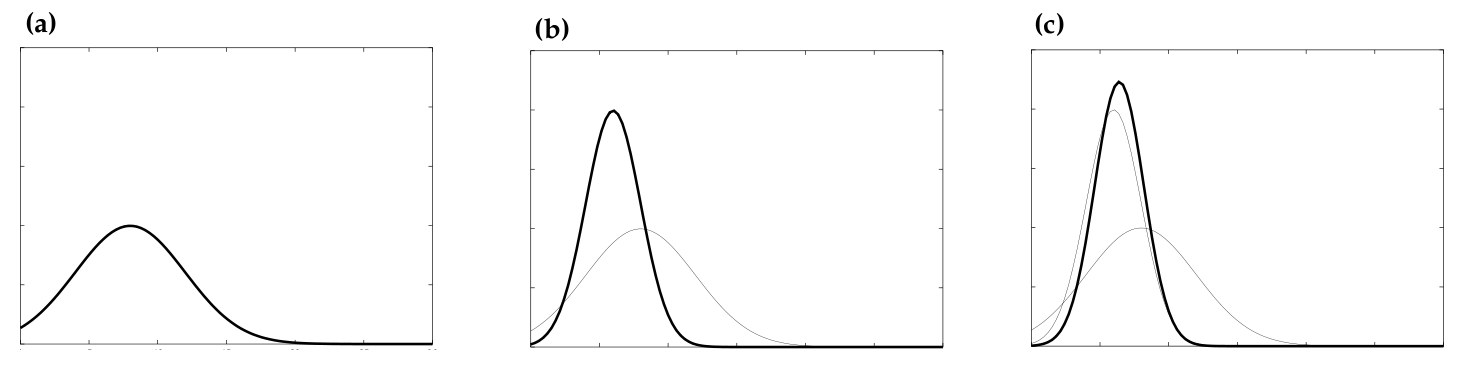
\includegraphics[width=\textwidth]{kalman}
    \caption{UKF: (a) Initial Belief  (b) Noisy Measurement  (c) incorporated into the belief. \cite{Thrun2005}}
    \end{figure}
    \end{column}
    \end{columns}
\end{itemize}
\end{frame}

\subsection{Particle Filter}
%frame with example
\begin{frame}{Example System Identification}
\begin{itemize}
\item Given:
    \begin{itemize}
    \item Elevation Map (1D)
    \item Ability To Measure Elevation
    \end{itemize}
\item Particle Consists of the unknowns:
    \begin{itemize}
    \item State: Location  $[0, 20]$
    \item Constant: Direction  $\{Left, Right\}$
    \end{itemize}
\end{itemize}

\begin{center}
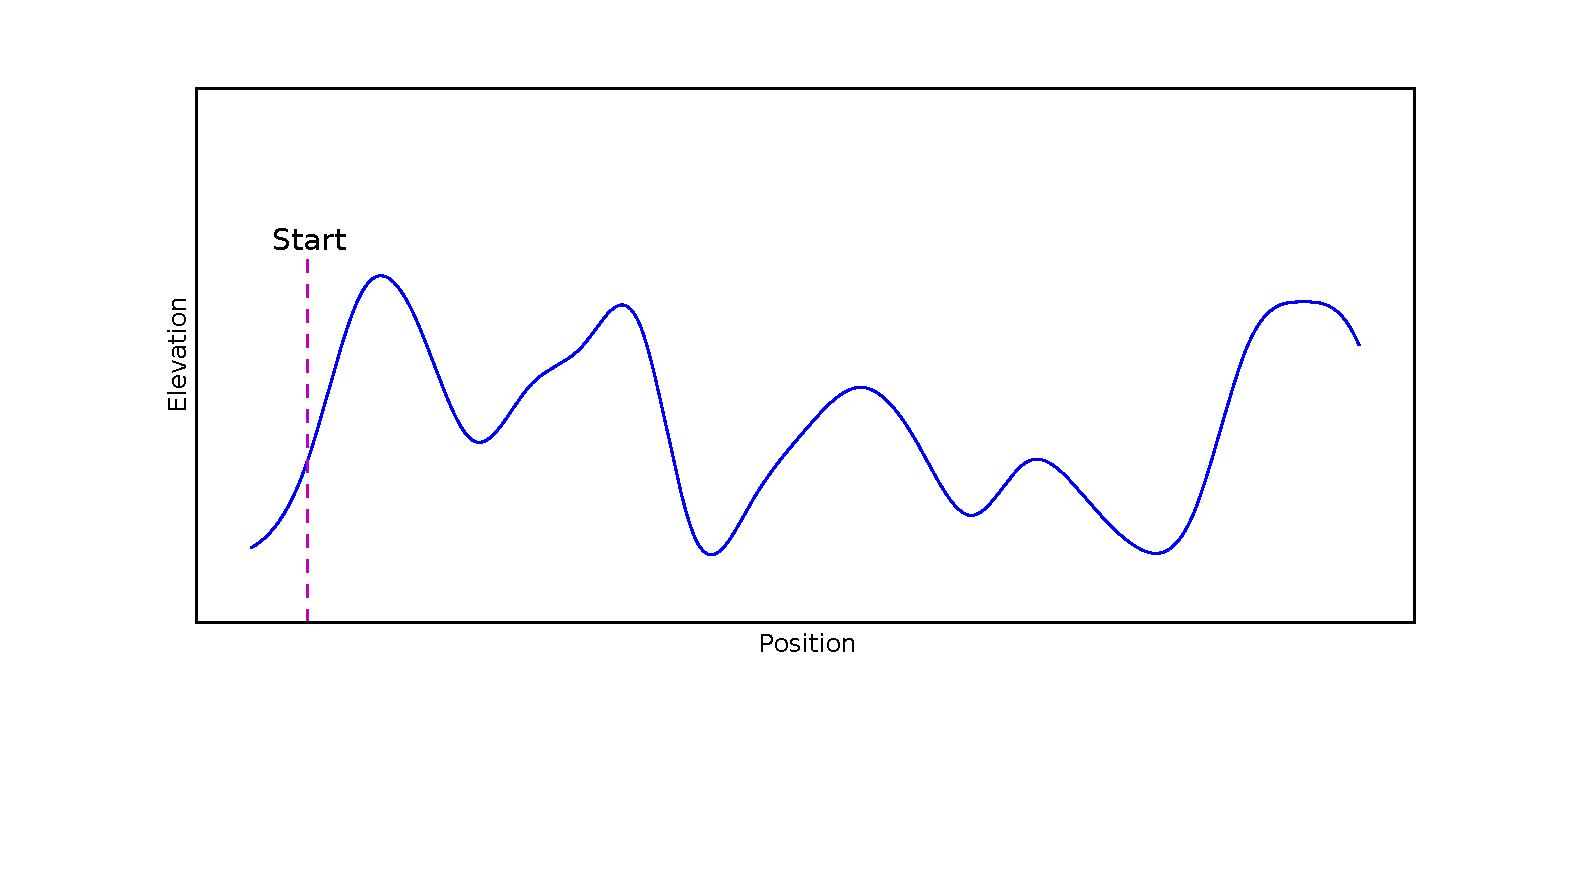
\includegraphics[clip=true,trim=2cm 3cm 3cm 3cm,width=.7\textwidth]{setup}
\end{center}
\end{frame}

\begin{frame}{Initial Distribution}
\centering
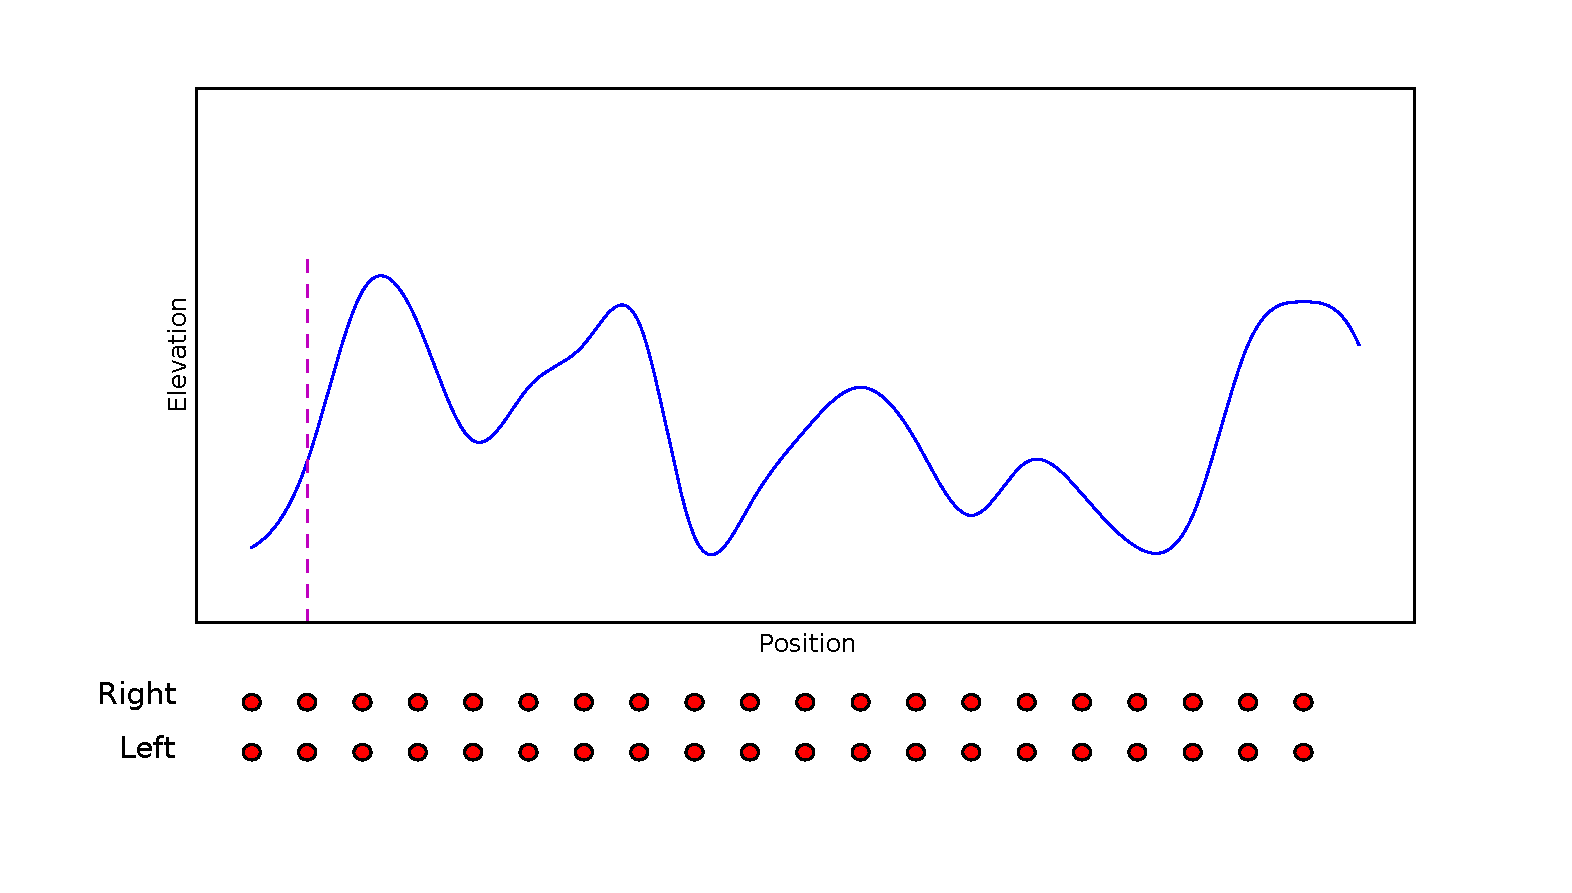
\includegraphics[width=\textwidth]{init}\\
\end{frame}

\begin{frame}{Measurement 1}
\centering
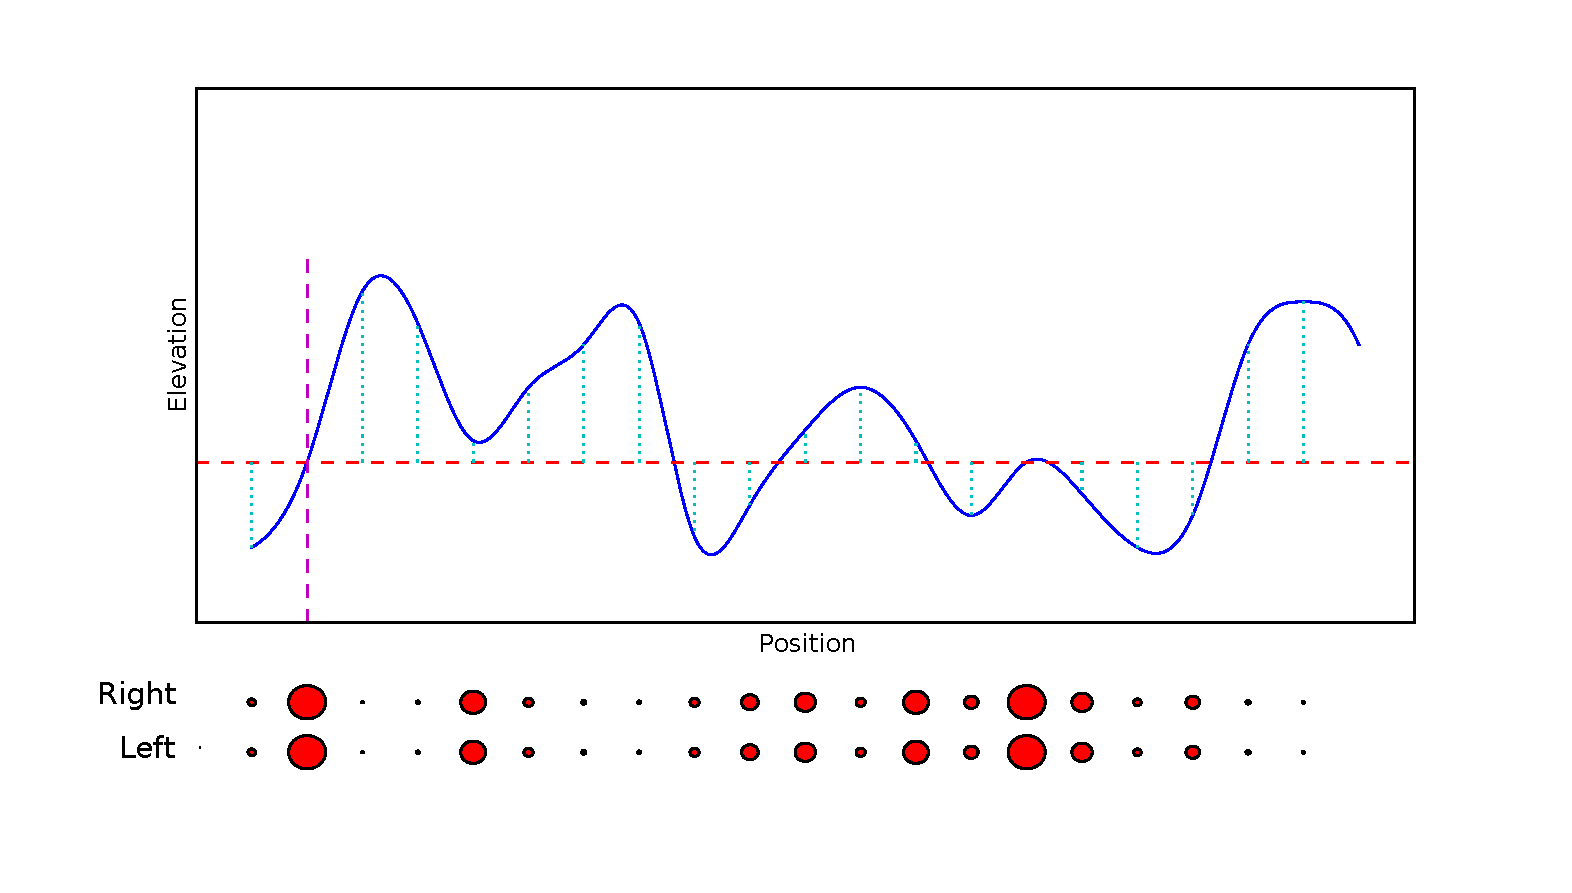
\includegraphics[width=\textwidth]{meas1}\\
\end{frame}

\begin{frame}{Step Forward}
\centering
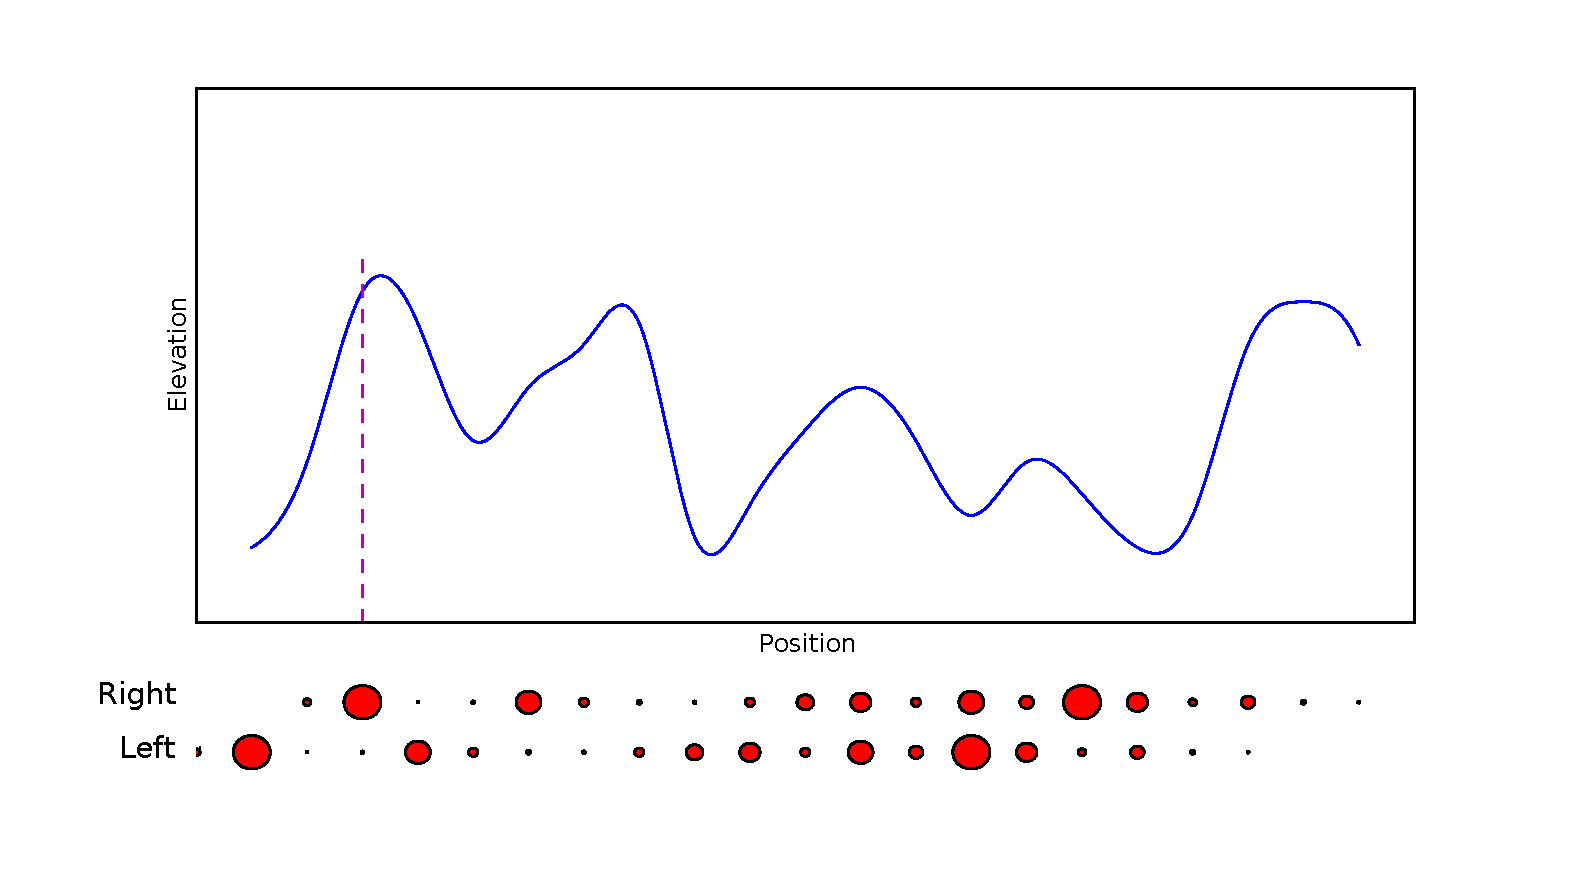
\includegraphics[width=\textwidth]{move1}\\
\end{frame}

\begin{frame}{Measurement 2}
\centering
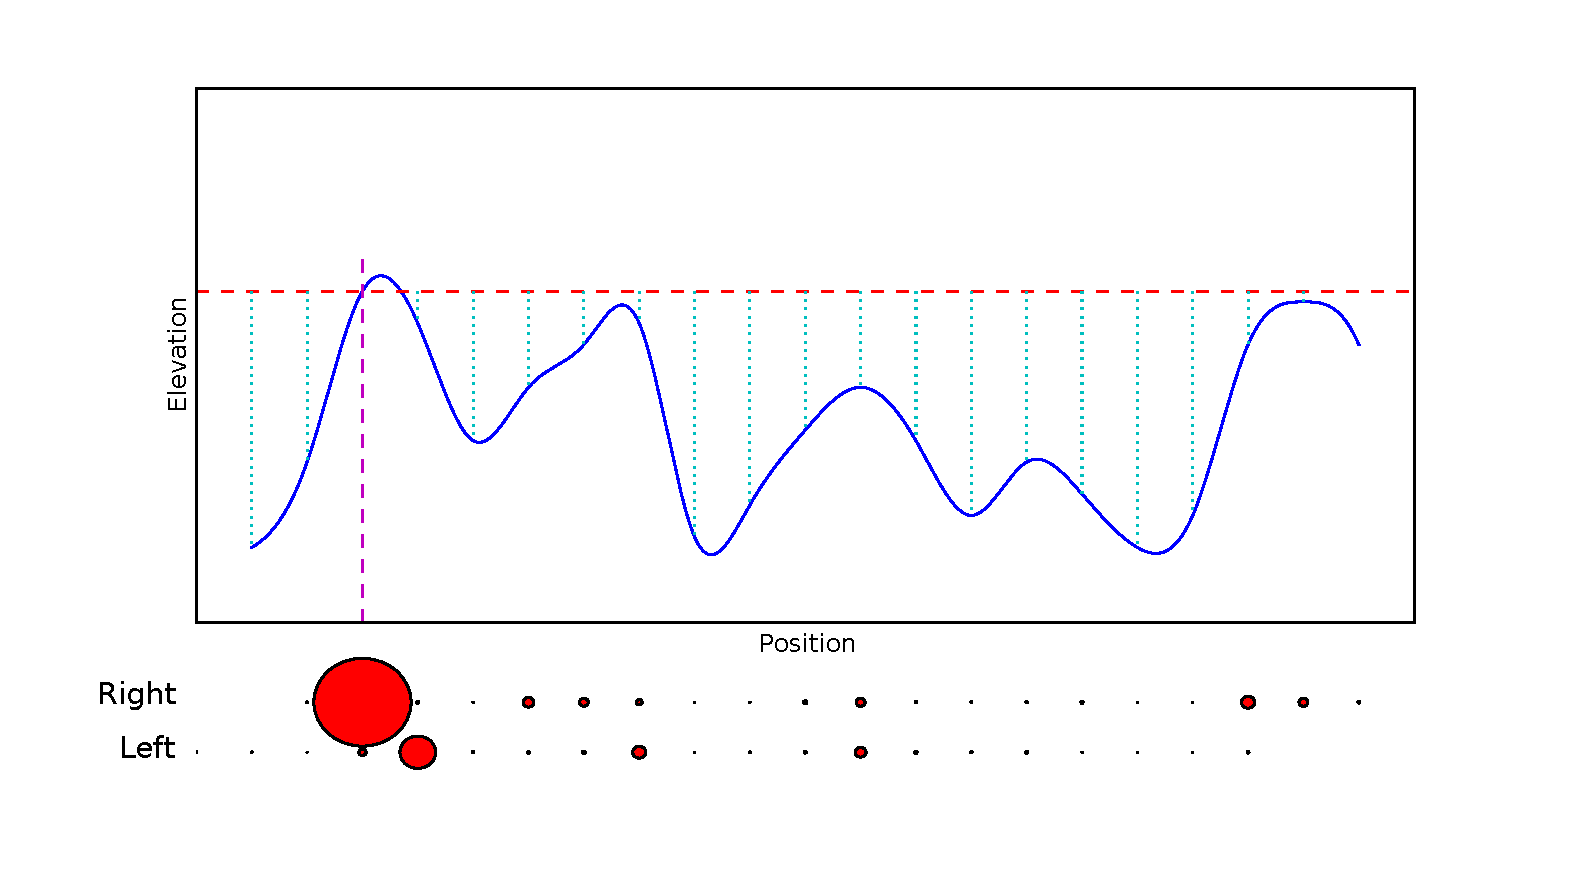
\includegraphics[width=\textwidth]{meas2}\\
\end{frame}

\begin{frame}{Step Forward}
\centering
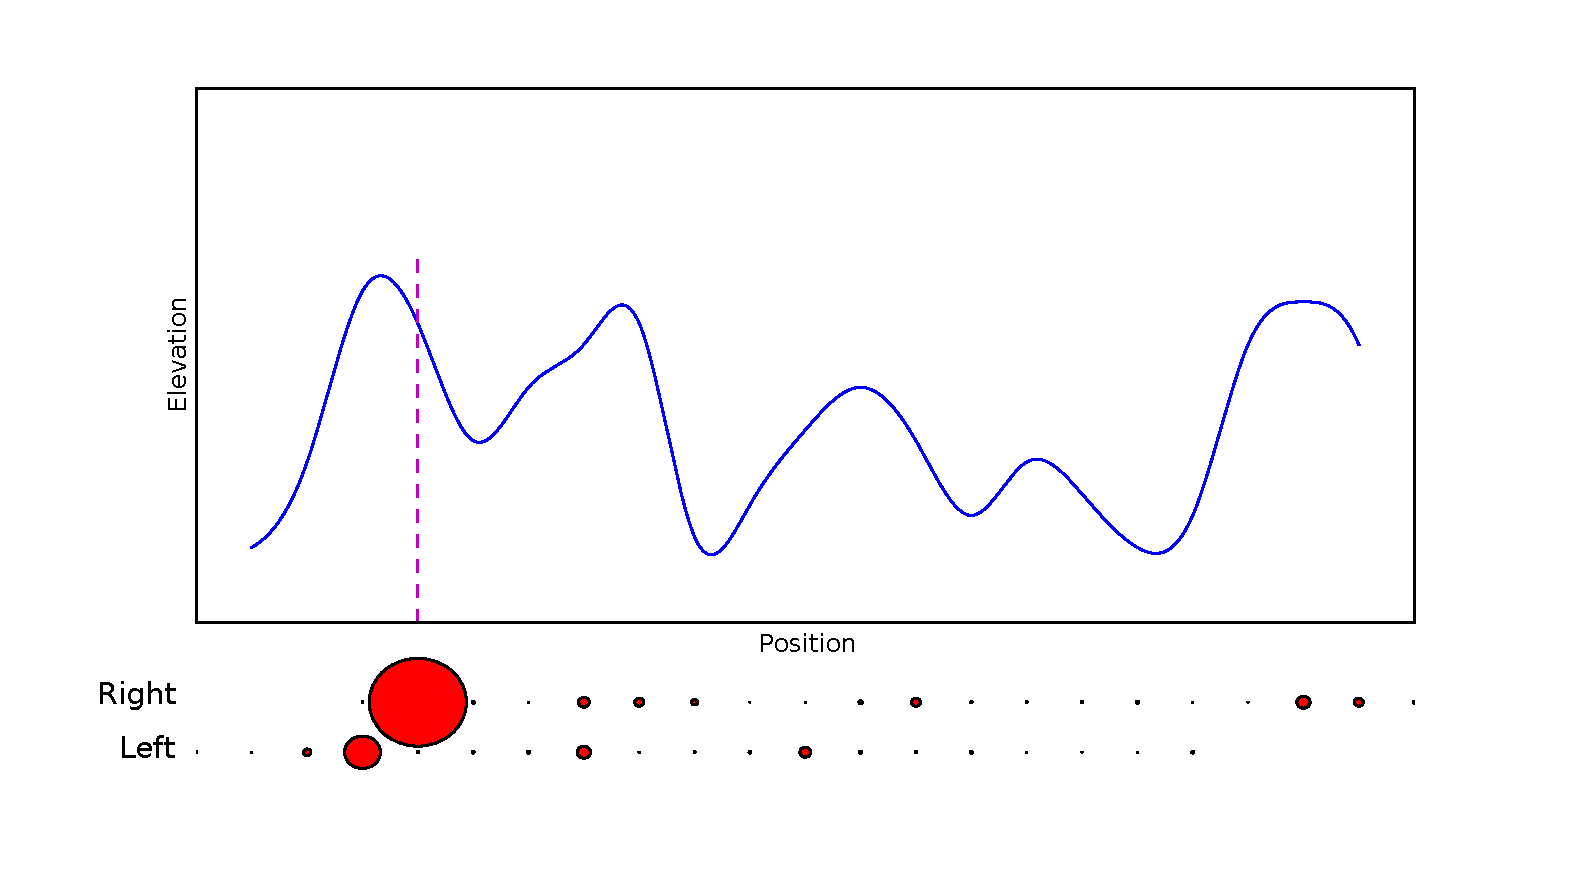
\includegraphics[width=\textwidth]{move2}\\
\end{frame}

\begin{frame}{Particle Filter Concepts}
\small
\begin{columns}
\begin{column}{.5\textwidth}
\begin{itemize}
    \item Weighting Function
    \item Resampling
    \begin{itemize}
        \item Remove Useless Particles
    \end{itemize}
    \item Regularized Resampling
    \begin{itemize}
        \item Prevent Redundant Particles
        \item Reduces Quantization Error
    \end{itemize}
\end{itemize}
\end{column}

\begin{column}{.5\textwidth}
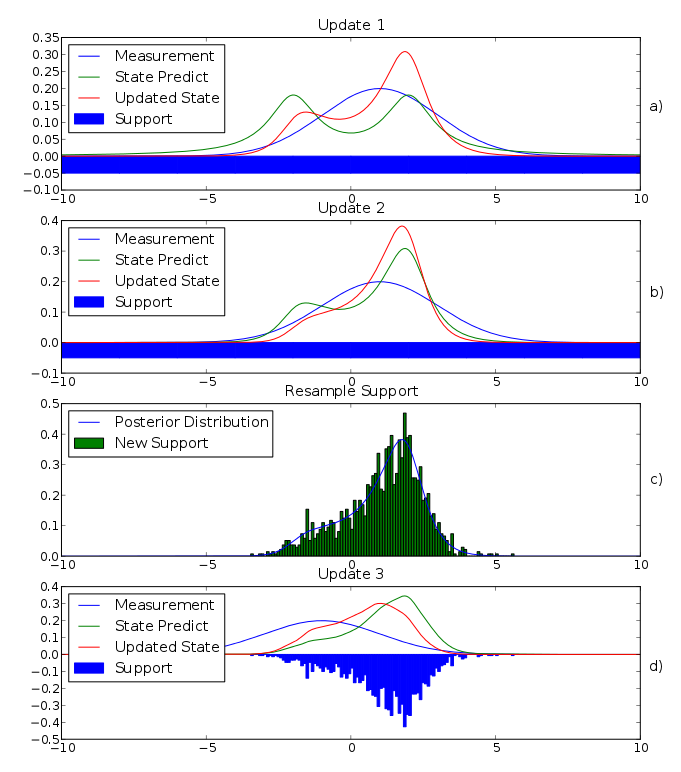
\includegraphics[clip=true,trim=0cm 6cm 0cm 6cm,width=\textwidth]{particle_filter2}
\end{column}
\end{columns}
\end{frame}

\begin{frame}{Construction}
\begin{itemize}
    \item Mixture PDF at time $k$, with $N_p$ particles:\\
        $$P(x_k) = \sum_{i=0}^{N_p} w^i\delta(x_k - x^i_k ) dx$$
    \item Weight of Particle $i$, at time $t_k$:\\
        $$w^i_k \propto \frac{P(x^i_{0:k} | y_{0:k})}{q(x^i_{0:k} | y_{0:k})}$$
      \note{$q$ is the density/location of the particle}
      \note{$p$ is the actual probability }
    \item Incorporating a Measurement, $y_k$:\\
        $$w^i_k \propto & w^i_{k-1}P(y_k| x_k) $$
      \note{Because of the proportion, note that the weights do not
            have to integrate to 1, and can be extremely large or extremely small}
\end{itemize}
\end{frame}
